% Chapter Template

\chapter{Dataset} % Main chapter title

\label{Chapter2_Dataset} % Change X to a consecutive number; for referencing this chapter elsewhere, use \ref{ChapterX}

\lhead{Chapter 2. \emph{Dataset}} % Change X to a consecutive number; this is for the header on each page - perhaps a shortened title

%----------------------------------------------------------------------------------------
%\tSECTION 1
%---------------------------------------------------------------------------------------
\section{nuScenes Dataset}

The nuScenes dataset \citep{caesar2020nuscenes} is a large-scale, multi-modal dataset for autonomous driving, developed by Motional (formerly nuTonomy). It was the first dataset to feature a full autonomous vehicle sensor suite, including 6 cameras, 5 radars, and 1 lidar, all with a full 360-degree field of view. This comprehensive sensor setup provides a rich and holistic view of the environment, which is crucial for developing robust perception systems.

\subsection{Sensor Suite}
The sensor setup, as detailed in Table \ref{tab:nuscenes_sensors}, is critical for our project. The BEVDepth model, which we use for scene understanding, is designed to consume images from all 6 cameras. The Lidar and Radar data provide ground-truth depth and velocity information, which, while not used as direct model inputs, are foundational to the dataset's ground-truth annotations.

\begin{table}[h]
\centering
\caption{nuScenes Sensor Specifications. (Adapted from \citep{caesar2020nuscenes})}
\label{tab:nuscenes_sensors}
\begin{tabular}{l p{9cm}}
\hline
\textbf{Sensor} & \textbf{Details} \\
\hline
6x Camera & RGB, 12Hz capture, $1600 \times 900$ resolution, 360° coverage. \\
1x Lidar & 32-beam, 20Hz capture, 360° horizontal FOV, $\le 70m$ range. \\
5x Radar & 77GHz, 13Hz capture, $\le 250m$ range, provides velocity. \\
GPS \& IMU & For localization and sensor synchronization. \\
\hline
\end{tabular}
\end{table}

\subsection{Data Collection}

The data was collected in Boston and Singapore, two cities known for their dense traffic and challenging driving scenarios. The dataset comprises 1000 scenes, each 20 seconds long. These scenes were carefully selected to include a wide variety of interesting and challenging situations, such as high traffic density, rare object classes, and complex maneuvers. The dataset is split into 700 scenes for training, 150 for validation, and 150 for testing. The dataset is also notable for its inclusion of diverse weather and lighting, with 19.4\% of scenes captured in the rain and 11.6\% at night.

\subsection{Annotations}

nuScenes provides detailed annotations for 23 object classes, including various types of vehicles, pedestrians, and cyclists. The annotations consist of 3D bounding boxes, instance masks, and 8 attributes, such as visibility, activity, and pose. With 7 times more annotations and 100 times more images than the pioneering KITTI dataset, nuScenes represents a significant leap forward in terms of data volume and complexity. The dataset also includes a high-definition map with 11 semantic layers, providing crucial contextual information for scene understanding.

\subsection{Significance and Impact}

The release of the nuScenes dataset has had a significant impact on the autonomous driving research community. It has enabled the development and evaluation of a wide range of algorithms for tasks such as 3D object detection, tracking, and motion forecasting. The dataset's design is uniquely suited to the methodology of this thesis. The 360° camera suite is a prerequisite for BEVDepth, which generates a dense Bird's-Eye-View (BEV) feature map from these multi-view images. Furthermore, the 20-second-long scenes provide the rich, long-term trajectory histories necessary to train and evaluate the AgentFormer motion forecasting model.

\begin{figure}[h]
\centering
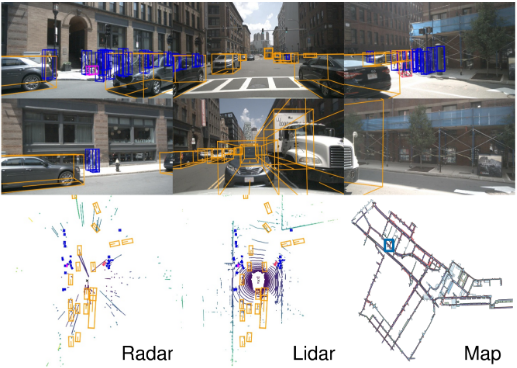
\includegraphics[width=\textwidth]{nuscenes_teaser.png}
\caption{A sample from the nuScenes dataset, showing the 6 camera views (top), along with Lidar and Radar point clouds (bottom left/middle) and the semantic map (bottom right). This full sensor suite provides a comprehensive view of the driving scene. (Image from \citep{caesar2020nuscenes})}
\label{fig:nuscenes_teaser}
\end{figure}

\begin{figure}[h]
\centering
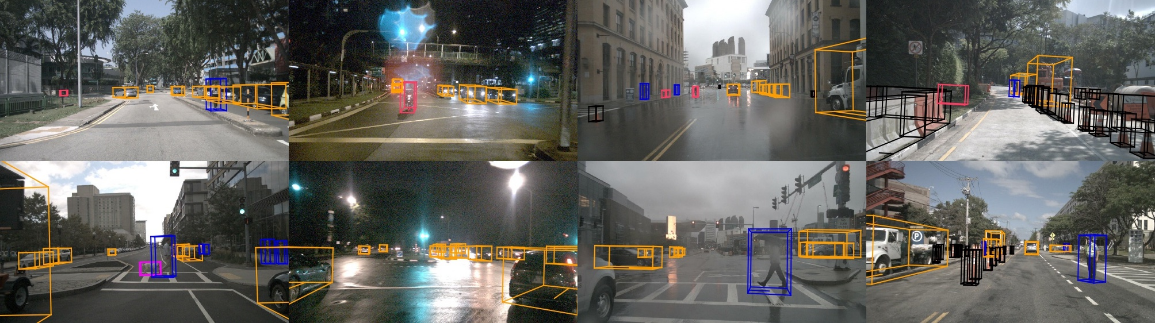
\includegraphics[width=\textwidth]{nuscenes_conditions.png}
\caption{Examples of the diverse conditions in nuScenes, including: (col 1) clear weather, (col 2) nighttime, (col 3) rain, and (col 4) construction zones. (Image from \citep{caesar2020nuscenes})}
\label{fig:nuscenes_conditions}
\end{figure}


